% ============================================================
% PowDev Workshop Presentation
% ============================================================
\documentclass[aspectratio=169, 10pt]{beamer}
\usetheme{metropolis}
\usepackage{appendixnumberbeamer}

\definecolor{powBlue}{RGB}{52, 152, 219}
\definecolor{powRed}{RGB}{231, 76, 60}
\definecolor{powGreen}{RGB}{46, 204, 113}
\definecolor{powPurple}{RGB}{155, 89, 182}
\definecolor{powOrange}{RGB}{243, 156, 18}
\definecolor{powTeal}{RGB}{26, 188, 156}
\definecolor{powPink}{RGB}{233, 30, 99}
\definecolor{powBrown}{RGB}{121, 85, 72}
\definecolor{powGray}{RGB}{96, 125, 139}

\setbeamercolor{frametitle}{bg=powBlue!90!black, fg=white}
\setbeamercolor{progress bar}{fg=powOrange}
\setbeamercolor{alerted text}{fg=powRed}

\usepackage[T1]{fontenc}
\usepackage[utf8]{inputenc}
\usepackage{lmodern}
\usepackage{amsmath, amssymb}
\usepackage{booktabs}
\usepackage{multirow}
\usepackage{graphicx}
\graphicspath{{./}{..}}
\usepackage{tikz}
\usetikzlibrary{shapes.geometric, arrows.meta, positioning, shadows, calc, fit, backgrounds}
\usepackage{xcolor}
\usepackage{array}
\usepackage{hyperref}

\newcommand{\highlight}[1]{\textcolor{powOrange}{\textbf{#1}}}

% Two-way appendix navigation
\newcommand{\applink}[2]{\hyperlink{#1}{\beamergotobutton{\tiny #2}}}
\newcommand{\backlink}[2]{\vfill\hfill\hyperlink{#1}{\beamerreturnbutton{\tiny #2}}}

\title{Coordinating Multilayer Power System Flexibility}
\subtitle{A Hybrid MILP--GNN--EBM Framework\\for Large-Scale Scenario Exploration}
\author{Th\'eotime Coudray \and St\'ephane Goutte}
\institute{UVSQ -- UMI SOURCE -- Projet PowDev}
\date{Workshop PowDev -- 2025}

\begin{document}

% ============================================================
\begin{frame}[plain]
  \titlepage
\end{frame}

\begin{frame}{Outline}
  \tableofcontents
\end{frame}

% %%%%%%%%%%%%%%%%%%%%%%%%%%%%%%%%%%%%%%%%%%%%%%%%%%%%%%%%%%%%
\section{Context \& Motivations}
% %%%%%%%%%%%%%%%%%%%%%%%%%%%%%%%%%%%%%%%%%%%%%%%%%%%%%%%%%%%%

\begin{frame}{The Challenge: Multi-Scale Flexibility under Stress}
\begin{columns}[T]
\begin{column}{0.55\textwidth}
\textbf{Power systems are transforming:}
\begin{itemize}
  \item Massive variable renewables (VRE) integration
  \item Distributed flexibility: storage, demand response, cross-border exchanges
  \item Growing \highlight{extreme events}: heat waves, wind droughts, cascading failures
\end{itemize}
\vspace{0.5em}
\textbf{Stakeholders no longer ask one question}\\[2pt]
\emph{``What is the optimal schedule today?''}\\[4pt]
\textbf{They need thousands of \emph{what-if} scenarios}\\[2pt]
\emph{Extreme weather, topology changes, new flexibility portfolios\ldots}
\end{column}
\begin{column}{0.42\textwidth}
\centering
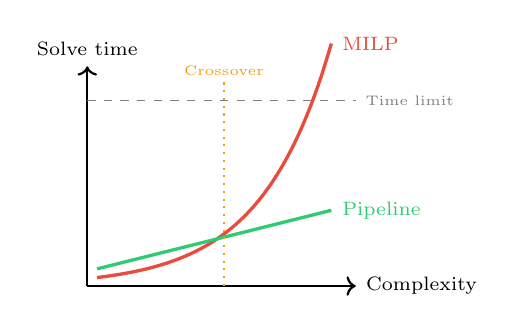
\begin{tikzpicture}[scale=0.62, every node/.style={font=\scriptsize}]
  \draw[->, thick] (0,0) -- (5.5,0) node[right] {Complexity};
  \draw[->, thick] (0,0) -- (0,4.5) node[above] {Solve time};
  \draw[powRed, very thick] plot[smooth, domain=0.2:5] (\x, {0.15*exp(0.7*\x)}) node[right] {MILP};
  \draw[powGreen, very thick] plot[smooth, domain=0.2:5] (\x, {0.3+0.25*\x}) node[right] {Pipeline};
  \draw[dashed, gray] (0,3.8) -- (5.5,3.8) node[right, font=\tiny] {Time limit};
  \draw[dotted, powOrange, thick] (2.8,0) -- (2.8,4.2);
  \node[font=\tiny, powOrange] at (2.8, 4.4) {Crossover};
\end{tikzpicture}
\vspace{0.3em}
{\scriptsize \textit{MILP scales exponentially; pipeline scales sub-linearly.}}
\end{column}
\end{columns}
\end{frame}

\begin{frame}{Literature Landscape \& Research Gap}
\begin{columns}[T]
\begin{column}{0.48\textwidth}
\textbf{MILP: the reference tool}
\begin{itemize}
  \item Rigorous, auditable, economically meaningful
  \item Multi-layer formulations exist\\{\scriptsize (Conejo 2016, Marquant 2017, Yokoyama 2021)}
  \item \alert{But:} exponential cost for large scenario sweeps
\end{itemize}
\vspace{0.4em}
\textbf{GNN surrogates}
\begin{itemize}
  \item Topology-aware, fast inference\\{\scriptsize (Donon 2019, Liu 2023, Deihim 2024)}
  \item \alert{But:} hard to guarantee feasibility
\end{itemize}
\end{column}
\begin{column}{0.48\textwidth}
\textbf{Energy-Based Models (EBMs)}
\begin{itemize}
  \item Exploration of discrete spaces\\{\scriptsize (Sun 2022, Goshvadi 2023)}
  \item \alert{But:} rarely applied to power system UC
\end{itemize}
\vspace{0.4em}
\textbf{\textcolor{powOrange}{Research gaps:}}
\begin{enumerate}
  \item Scenario exploration still solver-bound
  \item Surrogates lack end-to-end feasibility
  \item No controlled exploration of discrete spaces
  \item Weak coupling with economic signals
  \item No interactive near-real-time what-if tools
\end{enumerate}
\end{column}
\end{columns}
\end{frame}

% %%%%%%%%%%%%%%%%%%%%%%%%%%%%%%%%%%%%%%%%%%%%%%%%%%%%%%%%%%%%
\section{Research Question}
% %%%%%%%%%%%%%%%%%%%%%%%%%%%%%%%%%%%%%%%%%%%%%%%%%%%%%%%%%%%%

\begin{frame}{Research Question}
\begin{center}
\Large
\textit{Can a hybrid \highlight{MILP--GNN--EBM} methodology enable\\[6pt]
\highlight{near-real-time exploration} of multi-scale flexibility scenarios\\[6pt]
---and remain effective as scenarios become \highlight{increasingly complex}?}
\end{center}
\vspace{1em}
\begin{columns}[T]
\begin{column}{0.3\textwidth}
\centering\textbf{\textcolor{powRed}{MILP}}\\[4pt]{\small Rigour \& auditability\\Ground-truth labels}
\end{column}
\begin{column}{0.3\textwidth}
\centering\textbf{\textcolor{powPurple}{GNN}}\\[4pt]{\small Topology awareness\\Compact embeddings}
\end{column}
\begin{column}{0.3\textwidth}
\centering\textbf{\textcolor{powOrange}{EBM}}\\[4pt]{\small Controlled exploration\\Multi-candidate sampling}
\end{column}
\end{columns}
\end{frame}

% %%%%%%%%%%%%%%%%%%%%%%%%%%%%%%%%%%%%%%%%%%%%%%%%%%%%%%%%%%%%
\section{Method Overview}
% %%%%%%%%%%%%%%%%%%%%%%%%%%%%%%%%%%%%%%%%%%%%%%%%%%%%%%%%%%%%

\begin{frame}{Methodology Overview: The Reconstruct-then-Optimize Pipeline}
    \centering
    \includegraphics[width=\textwidth, height=0.8\textheight, keepaspectratio]{fig0_pipeline_overview.png}
\end{frame}

% %%%%%%%%%%%%%%%%%%%%%%%%%%%%%%%%%%%%%%%%%%%%%%%%%%%%%%%%%%%%
\section{Methodology: Building Blocks}
% %%%%%%%%%%%%%%%%%%%%%%%%%%%%%%%%%%%%%%%%%%%%%%%%%%%%%%%%%%%%

\begin{frame}{Block 1: Scenario Generator}
\hypertarget{main:scengen}{}
\begin{columns}[T]
\begin{column}{0.45\textwidth}
\textbf{Goal:} Generate diverse, tractable what-if instances.
\vspace{0.2em}

Each scenario $s = (\mathcal{G}, \mathcal{A}, \pi, \tau, c, \xi)$:
\begin{itemize}
  \item \textbf{Network} $\mathcal{G}$: regions, zones, interties
  \item \textbf{Assets} $\mathcal{A}$: thermal, nuclear, solar, wind, battery, DR, pumped hydro
  \item \textbf{Policy} $\pi$: CO$_2$ price, cross-border rules
  \item \textbf{Exogenous} $\xi$: weather, demand, hydro inflows
\end{itemize}
\vspace{0.2em}
\textbf{Three mechanisms:}
\begin{enumerate}
  \item \textbf{Budget guard} -- rejects intractable
  \item \textbf{LHS + $k$-center} -- max diversity
  \item \textbf{Criticality index}\\$\mathrm{Crit}(s) = \alpha\,\mathrm{Stress} + (1{-}\alpha)\,\mathrm{Hard}$
\end{enumerate}
\end{column}
\begin{column}{0.53\textwidth}
\centering
\vspace{4em}

\includegraphics[width=\textwidth]{scenario_paper_figure.png}
{\footnotesize{Two illustrative realizations of the scenario generator.}}
\vspace{4em}

{\tiny Low-criticality (left) vs.\ high-criticality (right): capacity portfolios and demand profiles.}
\end{column}
\end{columns}
\vspace{0.2em}
\applink{app:L}{App.~L: Criticality}
\applink{app:W}{App.~W: Scenarios}
\applink{app:X}{App.~X: Simple}
\applink{app:Y}{App.~Y: Critical}
\end{frame}

\begin{frame}{Block 2: Multi-Scale MILP Oracle}
\hypertarget{main:milp}{}
\begin{columns}[T]
\begin{column}{0.50\textwidth}
\textbf{Multi-period UC + economic dispatch}\\[4pt]
Coordinates all flexibility resources:
\begin{itemize}
  \item Thermal commitment \& startup
  \item Nuclear baseload (must-run)
  \item Battery \& pumped-hydro storage
  \item Demand response (multi-tier)
  \item Cross-border import/export
  \item Renewable curtailment
\end{itemize}
\vspace{0.3em}
\textbf{Objective:} Minimise total cost\\
{\small $\min_{u,x}\; C^{\mathrm{gen}} + C^{\mathrm{su}} + C^{\mathrm{dr}} + C^{\mathrm{uns}} + C^{\mathrm{spl}} + C^{\mathrm{sto}} + C^{\mathrm{imp}} + C^{\mathrm{ovg}}$}
\vspace{0.3em}

\textbf{9 constraint families}\\
{\scriptsize Thermal UC, nuclear, VRE, DR, battery, reservoir, pumped-hydro, transmission, nodal balance}
\end{column}
\begin{column}{0.46\textwidth}
\textbf{Key design choices:}
\vspace{0.3em}
\begin{itemize}
  \item \highlight{Binary variables} $u$: commitment, modes -- the \emph{hard} decisions
  \item \textbf{Continuous variables} $x$: dispatch, SOC, flows -- recovered later by LP
\end{itemize}
\vspace{0.4em}
\textbf{Label quality:}
\begin{itemize}
  \item \textcolor{powGreen}{\textbf{Gold}}: solved to optimality (4,388)
  \item \textcolor{powOrange}{\textbf{Silver}}: best incumbent at time limit (612)
  \item \applink{app:Y}{Dispatch comparison}
\end{itemize}
\vspace{0.4em}
\textbf{Scale:} 5,000 training scenarios\\
$\sim$45k--139k variables per instance\\
Solve time: seconds to hours
\end{column}
\end{columns}
\vspace{0.1em}
\applink{app:A}{App.~A: Objective}
\applink{app:B}{App.~B: Variables}
\applink{app:C}{App.~C: Constraints}
\end{frame}

\begin{frame}{Block 3: Graph Builder \& Hierarchical Temporal Encoder}
\hypertarget{main:hte}{}
\begin{columns}[T]
\begin{column}{0.48\textwidth}
\textbf{Why a graph?}
\begin{itemize}
  \item Variable size (4--160 zones)
  \item Explicit topology: containment + transmission
  \item Temporal coupling: SOC, ramps, DR cooldowns
\end{itemize}
\vspace{0.2em}
\textbf{Heterogeneous temporal graph:}
\begin{itemize}
  \item \textbf{5 node types:} nation, region, zone, asset, weather
  \item \textbf{11 edge types:} 7 spatial + 4 temporal
  \item Supra-graph: $N_{\mathrm{base}} \times T$ nodes
\end{itemize}
\vspace{0.2em}
\textbf{No MILP solution needed} $\to$ usable at inference
\end{column}
\begin{column}{0.48\textwidth}
\textbf{Hierarchical Temporal Encoder (HTE):}
\vspace{0.2em}

Three-phase architecture:
\begin{enumerate}
  \item \textbf{Bottom-up:} assets $\to$ zones $\to$ regions $\to$ nation\\{\scriptsize (graph attention + pooling)}
  \item \textbf{Temporal Transformer} at nation level\\{\scriptsize (self-attention over $T$ steps)}
  \item \textbf{Top-down:} broadcast + skip connections
\end{enumerate}
\vspace{0.3em}
\highlight{Self-supervised training:}\\
{\small InfoNCE contrastive, multi-lag ($\tau \in \{1,4,8\}$h).\\
\textbf{No MILP labels required.}}
\vspace{0.2em}

Output: $h \in \mathbb{R}^{Z \times T \times 128}$\\
{\scriptsize 3.2M params, $\sim$8h training on A100}
\end{column}
\end{columns}
\vspace{0.1em}
\applink{app:W}{App.~W: Scenarios}
\applink{app:AA}{App.~AA: Graph}
\applink{app:AB}{App.~AB: HTE}
\end{frame}

\begin{frame}{Block 4: Energy-Based Model \& Langevin Sampler}
\hypertarget{main:ebm}{}
\begin{columns}[T]
\begin{column}{0.48\textwidth}
\textbf{Why an EBM?}
\begin{enumerate}
  \item \textbf{Multimodality:} multiple near-optimal schedules -- captures full landscape
  \item \textbf{Controlled exploration:} Langevin dynamics with tunable temperature
  \item \textbf{Downstream compatible:} relaxed in training, binary at inference
\end{enumerate}
\vspace{0.2em}
\textbf{Architecture:}
\begin{itemize}
  \item Input: $u \in \{0,1\}^{Z \times T \times 7}$ + embedding $h$
  \item Bidirectional GRU + energy head
  \item Mean energy + \highlight{peak energy} (log-sum-exp)
  \item Zone masking for variable sizes
\end{itemize}
\end{column}
\begin{column}{0.48\textwidth}
\textbf{Langevin Sampling (logit space):}
\vspace{0.2em}

{\small $z^{(k+1)} \leftarrow z^{(k)} - \eta\nabla_z E_\theta(\sigma(z^{(k)}), h) + \sigma_k\sqrt{\eta}\,\varepsilon_k$}
\vspace{0.2em}

{\small Temperature annealing: broad $\to$ refined.\\
100 steps at inference, 10--50 during training.}
\vspace{0.4em}

\textbf{Two-step training:}
\begin{itemize}
  \item \textbf{Step A -- Gold pre-training:}\\
  Contrastive divergence (CD)\\
  {\scriptsize Push down MILP solutions, push up random}
  \item \textbf{Step B -- Silver fine-tuning:}\\
  Preference loss (LP-evaluated)\\
  {\scriptsize $\mathcal{L}_{\mathrm{pref}} = \max(0, E(u_a) - E(u_b) + \delta)$}\\
  {\scriptsize Aligns energy $\Leftrightarrow$ economic cost}
\end{itemize}
\end{column}
\end{columns}
\vspace{0.1em}
\applink{app:D}{App.~D: Binary repr.}
\applink{app:E}{App.~E: Langevin}
\applink{app:F}{App.~F: Training}
\end{frame}

\begin{frame}{Block 5: Solution Reconstruction \& Evaluation}
\hypertarget{main:recon}{}
\begin{columns}[T]
\begin{column}{0.48\textwidth}
\textbf{Feasibility Decoder (heuristic):}
\begin{enumerate}
  \item \textbf{Phase 1:} Must-run (nuclear, VRE)
  \item \textbf{Phase 2:} Deficit -- EBM-guided first, then merit-order\\
  {\scriptsize storage $\to$ thermal $\to$ imports $\to$ DR $\to$ unserved}
  \item \textbf{Phase 3:} Surplus -- exports $\to$ curtail $\to$ charge
\end{enumerate}
\vspace{0.2em}
\highlight{Trust the EBM first, guarantee feasibility always.}
\vspace{0.3em}

\textbf{Two-Stage LP Worker:}\\
{\small Fixes binaries $\to$ solves continuous LP.\\
Progressive repair: hard-fix $\to$ repair-20 $\to$ repair-100 $\to$ full-soft $\to$ round \& refix}
\end{column}
\begin{column}{0.48\textwidth}
\textbf{Evaluation protocol:}
\vspace{0.2em}

300 out-of-sample scenarios, 3 families:
\begin{itemize}
  \item \textbf{Low} ($\bar{C}=0.33$): 4--20 zones
  \item \textbf{Medium} ($\bar{C}=0.41$): 30--80 zones
  \item \textbf{High} ($\bar{C}=0.49$): 80--160 zones
\end{itemize}
\vspace{0.2em}
\textbf{Inference:} best-of-5 Langevin chains
\vspace{0.2em}

\textbf{Metrics:}
\begin{itemize}
  \item \textbf{Cost gap} (\%): $(C_\text{pipe} - C_\text{MILP}) / |C_\text{MILP}|$
  \item \textbf{Speedup}: $T_\text{MILP} / T_\text{pipe}$
  \item \textbf{Feasibility} (slack MWh)
  \item \textbf{LP stage} used
\end{itemize}
{\scriptsize Hardware: A100 GPU, HiGHS, PyTorch 2.5}
\end{column}
\end{columns}
\vspace{0.1em}
\applink{app:G}{App.~G: LP stages}
\applink{app:Y}{App.~Y: Dispatch}
\end{frame}

% %%%%%%%%%%%%%%%%%%%%%%%%%%%%%%%%%%%%%%%%%%%%%%%%%%%%%%%%%%%%
\section{Results}
% %%%%%%%%%%%%%%%%%%%%%%%%%%%%%%%%%%%%%%%%%%%%%%%%%%%%%%%%%%%%

\begin{frame}{Results: Central Divergence}
\hypertarget{main:central}{}
\centering

\includegraphics[width=0.92\textwidth]{fig14_central_divergence.png}

{\scriptsize (A) Solve time vs complexity: MILP (red) vs pipeline (green). (B) Speedup vs criticality. (C) Cost gap envelope.}

\applink{app:P}{App.~P: Solve time}
\applink{app:T}{App.~T: Complexity}
\end{frame}

\begin{frame}{Results: Three Criticality Families}
\hypertarget{main:families}{}
\textbf{Central finding:} \emph{Pipeline advantage scales with scenario difficulty.}\\
{\scriptsize Spearman $\rho({\rm crit}, {\rm speedup}) = +0.224$ ($p < 10^{-4}$), $\rho({\rm zones}, {\rm speedup}) = +0.299$ ($p < 10^{-7}$).}
\vspace{0.3em}

\centering
{\small
\begin{tabular}{lrrrrrrr}
\toprule
\textbf{Family} & $n$ & \textbf{Med.\ gap} & \textbf{Gap IQR} & \textbf{Med.\ $S$} & \textbf{$S$ IQR} & \textbf{HF} & \textbf{Better} \\
 & & (\%) & (\%) & ($\times$) & ($\times$) & (\%) & (\%) \\
\midrule
Low & 100 & 12.6 & {[}0.7, 23.3{]} & 0.12 & {[}0.10, 0.14{]} & 90 & 3 \\
Medium & 100 & 18.5 & {[}$-$34.8, 40.2{]} & 0.46 & {[}0.06, 1.47{]} & 65 & 33 \\
High & 100 & \textbf{$-$0.04} & {[}$-$118, 36.9{]} & \textbf{0.88} & {[}0.07, 10.8{]} & 40 & \textbf{51} \\
\bottomrule
\end{tabular}
}
\vspace{0.3em}

\begin{columns}[T]
\begin{column}{0.32\textwidth}
\centering\textbf{\textcolor{powGreen}{Low}}\\{\scriptsize MILP fast ($<$2\,s). Pipeline overhead. 90\% hard-fix.}
\end{column}
\begin{column}{0.32\textwidth}
\centering\textbf{\textcolor{powOrange}{Medium}}\\{\scriptsize Transition zone. Mean speedup 3.4$\times$.}
\end{column}
\begin{column}{0.32\textwidth}
\centering\textbf{\textcolor{powRed}{High}}\\{\scriptsize Sweet spot. Gap $-$0.04\%. $11.5\times$ on time-limited.}
\end{column}
\end{columns}
\vspace{0.3em}
\textbf{100\% feasibility rate} across all 300 scenarios (slack $< 0.01$\,MWh).

\applink{app:H}{App.~H: Full results}
\applink{app:U}{App.~U: Dashboard}
\applink{app:Q}{App.~Q: Pareto}
\applink{app:R}{App.~R: Cumul.\ time}
\applink{app:S}{App.~S: Timing}
\end{frame}

\begin{frame}{Results: Persona-Based Evaluation}
\hypertarget{main:personas}{}
\textbf{Different stakeholders stress different aspects.} Three personas:
\vspace{0.3em}

\centering
{\small
\begin{tabular}{lcccccc}
\toprule
\textbf{Persona} & \textbf{Key stress} & \textbf{TL} & \textbf{Med.\ gap} & \textbf{Mean $S$} & \textbf{Better} & \textbf{HF} \\
 & & (\%) & (\%) & ($\times$) & (\%) & (\%) \\
\midrule
VRE / Battery & Storage, high VRE & 0 & 4.7 & 0.2 & 22 & 17 \\
Network Oper. & Congestion, trade & 49 & 30.0 & 5.5 & 31 & 36 \\
Mathematician & Combinat.\ hard. & 28 & $-$100.6 & 2.6 & 76 & 15 \\
\bottomrule
\end{tabular}
}
\vspace{0.4em}

\begin{columns}[T]
\begin{column}{0.32\textwidth}
\centering\textbf{\textcolor{powGreen}{VRE / Battery}}\\[3pt]
{\scriptsize Best quality: 4.7\% gap. MILP fast. Pipeline: feasibility + diversity.}
\end{column}
\begin{column}{0.32\textwidth}
\centering\textbf{\textcolor{powBlue}{Network Operator}}\\[3pt]
{\scriptsize 49\% MILP time-outs. $5.5\times$ speedup. Pipeline's \highlight{strongest case}.}
\end{column}
\begin{column}{0.32\textwidth}
\centering\textbf{\textcolor{powPurple}{Mathematician}}\\[3pt]
{\scriptsize 76\% pipeline wins. MILP incumbents weak. But 77\% full-soft.}
\end{column}
\end{columns}
\vspace{0.3em}
$\Rightarrow$ \textbf{Persona-aware routing:} stress-dominated $\neq$ hardness-dominated.

\applink{app:M}{App.~M: Persona defs}
\applink{app:V}{App.~V: Persona dashboard}
\end{frame}

\begin{frame}{Persona Fingerprints}
\centering

\includegraphics[width=0.55\textwidth]{fig3_persona_radar.png}

{\scriptsize Radar chart of the 10 most discriminative criticality components across personas.\\Each vertex: normalised mean $\in [0,1]$ over 100 scenarios per persona.}
\end{frame}

\begin{frame}{Results: Out-of-Distribution (Extreme Criticality)}
\hypertarget{main:ood}{}
\textbf{100 extreme scenarios} above 95th pctl of training. \textbf{All 100 hit MILP time limit.}
\vspace{0.3em}

\centering
{\small
\begin{tabular}{lrr}
\toprule
\textbf{Metric} & \textbf{Extreme OOD} & \textbf{High ref.} \\
\midrule
MILP time-limited (\%) & 100 & 41 \\
Feasibility slack (MWh) & $<0.01$ & $<0.01$ \\
\midrule
Cost gap, median (\%) & 119.6 & $-$0.04 \\
Speedup, median ($\times$) & \textbf{5.4} & 0.88 \\
Pipeline time, median (s) & 223.4 & 247 \\
\midrule
Hard-fix (\%) & 48 & 40 \\
Full-soft (\%) & 6 & 53 \\
\bottomrule
\end{tabular}
}
\vspace{0.3em}

\begin{columns}[T]
\begin{column}{0.48\textwidth}
\textbf{\textcolor{powGreen}{Good news:}}
\begin{itemize}
  \item 100\% faster (median $5.4\times$, range $3.9$--$9.3\times$)
  \item 100\% feasible, near-zero slack
  \item 48\% hard-fix (EBM transfers well)
\end{itemize}
\end{column}
\begin{column}{0.48\textwidth}
\textbf{\textcolor{powRed}{Trade-off:}}
\begin{itemize}
  \item Cost gap 119.6\% (EBM under-represented)
  \item MILP also returns sub-optimal incumbents
  \item Feasible plans in $<$4 min even OOD
\end{itemize}
\end{column}
\end{columns}

\applink{app:I}{App.~I: Time-limited}
\applink{app:K}{App.~K: Failure modes}
\end{frame}

\begin{frame}{OOD: Robustness Analysis}
\hypertarget{main:robust}{}
\centering

\includegraphics[width=0.92\textwidth]{fig15_robustness_analysis.png}

{\scriptsize Robustness across extreme-criticality scenarios: solve time, cost gap, and pipeline timing.}
\end{frame}

% %%%%%%%%%%%%%%%%%%%%%%%%%%%%%%%%%%%%%%%%%%%%%%%%%%%%%%%%%%%%
\section{Conclusion}
% %%%%%%%%%%%%%%%%%%%%%%%%%%%%%%%%%%%%%%%%%%%%%%%%%%%%%%%%%%%%

\begin{frame}{Conclusion: Key Findings}
\hypertarget{main:conclusion}{}
\begin{enumerate}
  \item \textbf{Pipeline advantage scales with difficulty.}\\
  $\rho = +0.30$ (zones vs speedup). High-crit: gap $-$0.04\%, up to $11.5\times$ speedup.
  \vspace{0.3em}
  \item \textbf{100\% feasibility -- structural, not statistical.}\\
  Greedy decoder + LP progressive repair $\Rightarrow$ zero slack on all 300 scenarios.
  \vspace{0.3em}
  \item \textbf{EBM learns meaningful binary patterns.}\\
  65\% hard-fix rate (90\% on low-crit). Two-step training captures MILP logic.
  \vspace{0.3em}
  \item \textbf{Honest assessment:} 14.4\% median gap overall.\\
  MILP remains superior for easy scenarios ($<$2\,s). Pipeline valuable when MILP $>$60\,s.
  \vspace{0.3em}
  \item \textbf{Persona \& OOD robustness.}\\
  Performance varies by stress \emph{type}. Extreme scenarios: feasible in $<$4 min.
\end{enumerate}
\applink{app:J}{App.~J: Correlations}
\applink{app:O}{App.~O: Contributions}
\end{frame}

\begin{frame}{Limitations}
\hypertarget{main:limits}{}
\begin{columns}[T]
\begin{column}{0.48\textwidth}
\textbf{Methodological:}
\begin{itemize}
  \item[\textbf{L1}] \textbf{EBM generalisation to large topologies}\\{\scriptsize 53\% full-soft on high-crit -- few $>$100-zone training instances}
  \item[\textbf{L2}] \textbf{Greedy decoder sub-optimality}\\{\scriptsize No look-ahead; 12.6\% gap on easy scenarios}
  \item[\textbf{L3}] \textbf{Fixed pipeline overhead ($\sim$4\,s)}\\{\scriptsize Neural cost exceeds MILP for simple instances}
  \item[\textbf{L4}] \textbf{Single-horizon, deterministic}\\{\scriptsize No stochastic scenarios, no N$-$1 security}
\end{itemize}
\end{column}
\begin{column}{0.48\textwidth}
\textbf{Statistical \& validation:}
\begin{itemize}
  \item[\textbf{L5}] \textbf{Training distribution dependency}\\{\scriptsize All from same synthetic generator}
  \item[\textbf{L6}] \textbf{LP as scalability bottleneck}\\{\scriptsize $>$90\% time on high-crit is LP solve}
  \item[\textbf{L7}] \textbf{No real-world data}\\{\scriptsize Needs TSO validation}
\end{itemize}
\vspace{0.4em}
\textbf{Interpretation caveat:}\\
{\scriptsize Negative gaps on MILP-optimal scenarios are LP relaxation artefacts, not genuine superiority.}
\end{column}
\end{columns}
\end{frame}

\begin{frame}{Perspectives \& Next Steps}
\hypertarget{main:persp}{}
\begin{columns}[T]
\begin{column}{0.48\textwidth}
\textbf{Short-term:}
\begin{itemize}
  \item[\textbf{R1}] Scale EBM to larger topologies\\{\scriptsize Curriculum sampling + spatial attention}
  \item[\textbf{R2}] Learned decoder with look-ahead\\{\scriptsize End-to-end through LP cost signal}
  \item[\textbf{R4}] Batched GPU inference\\{\scriptsize Per-scenario cost $<$1\,s}
  \item[\textbf{R5}] Criticality-aware hybrid routing\\{\scriptsize MILP for easy, pipeline for hard}
\end{itemize}
\end{column}
\begin{column}{0.48\textwidth}
\textbf{Medium-term:}
\begin{itemize}
  \item[\textbf{R3}] Stochastic \& multi-period extensions
  \item[\textbf{R6}] Security constraints (N$-$1)
  \item[\textbf{R7}] Transfer across systems
\end{itemize}
\vspace{0.5em}
\highlight{Application paper (next):}\\[4pt]
\textbf{Extreme climate stress testing}\\
{\small Joint work with Anastasia.\\
Real climate-driven extreme scenarios as pipeline inputs. Validate on physically coherent projections.}
\applink{app:Zp}{App.~Z': Climate stress}
\end{column}
\end{columns}
\vspace{0.2em}
\applink{app:N}{App.~N: Economic advantage}
\vspace{0.4em}
\begin{center}
\textbf{The pipeline does not replace the MILP---it extends its reach\\to regimes where repeated exact solves are impractical.}
\end{center}
\end{frame}

\begin{frame}[standout]
  Thank you!\\\vspace{1em}{\normalsize Questions \& Discussion}\\\vspace{1em}{\small \texttt{theotime.coudray@uvsq.fr}}
\end{frame}

% %%%%%%%%%%%%%%%%%%%%%%%%%%%%%%%%%%%%%%%%%%%%%%%%%%%%%%%%%%%%
%                        APPENDICES
% %%%%%%%%%%%%%%%%%%%%%%%%%%%%%%%%%%%%%%%%%%%%%%%%%%%%%%%%%%%%
\appendix
\section*{Appendix and Supplementary Material}


\begin{frame}{App.\ A: MILP Objective Function}
\hypertarget{app:A}{}
\begin{equation*}
\min_{u,x} \; C^{\mathrm{gen}} + C^{\mathrm{su}} + C^{\mathrm{dr}} + C^{\mathrm{uns}} + C^{\mathrm{spl}} + C^{\mathrm{sto}} + C^{\mathrm{imp}} + C^{\mathrm{ovg}}
\end{equation*}
{\small
\begin{align*}
C^{\mathrm{gen}} &= \textstyle\sum_{z,t} ( c^{\mathrm{th}}_z p^{\mathrm{th}}_{z,t} + c^{\mathrm{nuc}}_z p^{\mathrm{nuc}}_{z,t} ) &
C^{\mathrm{su}} &= \textstyle\sum_{z,t} c^{\mathrm{su}}_z v^{\mathrm{th}}_{z,t} \\
C^{\mathrm{dr}} &= \textstyle\sum_{z,t,k} c^{\mathrm{dr}}_k d^{\mathrm{dr},k}_{z,t} &
C^{\mathrm{uns}} &= \textstyle\sum_{z,t} c^{\mathrm{voll}} q^{\mathrm{uns}}_{z,t} \\
C^{\mathrm{spl}} &= \textstyle\sum_{z,t} ( c^{\mathrm{res}} (s^{\mathrm{sol}} + s^{\mathrm{wnd}}) + c^{\mathrm{hsp}} h^{\mathrm{spl}} ) &
C^{\mathrm{sto}} &= \textstyle\sum_{z,t} c^{\mathrm{cyc}} (b^+ + b^- + g^+ + g^-) \\
C^{\mathrm{imp}} &= \textstyle\sum_{t} ( c^{\mathrm{imp}} m^+ + c^{\mathrm{exp}} m^- ) &
C^{\mathrm{ovg}} &= \textstyle\sum_{z,t} c^{\mathrm{ovg}} q^{\mathrm{ovg}}_{z,t}
\end{align*}
}
{\scriptsize $c^{\mathrm{th}}_z = c^{\mathrm{fuel}} + c^{\mathrm{marg}} + \pi_{\mathrm{CO}_2}\varepsilon$.\quad
DR tiers: $c^{\mathrm{dr}}_k = c^{\mathrm{dr}}_0 \cdot 1.5^k$.\quad
VOLL = last-resort penalty.}
\backlink{main:milp}{Block 2: MILP}
\end{frame}

\begin{frame}{App.\ B: MILP Decision Variables}
\hypertarget{app:B}{}
\begin{columns}[T]
\begin{column}{0.48\textwidth}
\textbf{Binary $u$:}
\begin{itemize}
  \item $u^{\mathrm{th}}_{z,t}$: thermal commitment
  \item $v^{\mathrm{th}}_{z,t}$: thermal startup
  \item $\delta^{\mathrm{dr}}_{z,t}$: DR activation
  \item $\sigma^{\mathrm{bat}}_{z,t}$: battery mode
  \item $\sigma^{\mathrm{phs}}_{z,t}$: pumped-hydro mode
  \item $\sigma^{\mathrm{imp}}_{t}$: import/export mode
\end{itemize}
{\scriptsize $\sim 4|\mathcal{Z}||\mathcal{T}| + |\mathcal{T}|$ before pre-fixing (reduces 30--60\%).}
\end{column}
\begin{column}{0.48\textwidth}
\textbf{Continuous $x$:}
\begin{itemize}
  \item $p^{\mathrm{th}}, p^{\mathrm{nuc}}, p^{\mathrm{sol}}, p^{\mathrm{wnd}}$: outputs
  \item $s^{\mathrm{sol}}, s^{\mathrm{wnd}}$: VRE curtailment
  \item $d^{\mathrm{dr}}, e^{\mathrm{dr}}$: DR shed \& rebound
  \item $b^+, b^-, e^{\mathrm{bat}}$: battery
  \item $g^+, g^-, e^{\mathrm{phs}}$: pumped-hydro
  \item $h^{\mathrm{rel}}, e^{\mathrm{hyd}}$: reservoir
  \item $f_{\ell,t}$: line flows
  \item $m^+, m^-$: cross-border
\end{itemize}
\end{column}
\end{columns}
\backlink{main:milp}{Block 2: MILP}
\end{frame}

\begin{frame}{App.\ C: MILP Constraint Families}
\hypertarget{app:C}{}
{\small
\begin{enumerate}
  \item \textbf{Thermal UC:} $\underline{P}^{\mathrm{th}} u^{\mathrm{th}} \leq p^{\mathrm{th}} \leq \overline{P}^{\mathrm{th}} u^{\mathrm{th}}$; ramp limits; startup detection
  \item \textbf{Nuclear:} must-run, modulation within capacity, ramp $R^{\mathrm{nuc}} = 0.5\overline{P}^{\mathrm{nuc}}$
  \item \textbf{Renewables:} dispatch = available $-$ curtailment
  \item \textbf{DR:} $K$ cost tiers, big-M activation, max activations, rebound with decay
  \item \textbf{Battery:} mutual exclusivity via $\sigma^{\mathrm{bat}}$; SOC: $e_t = \rho e_{t-1} + \eta^+ b^+ \Delta t - b^-\Delta t/\eta^-$
  \item \textbf{Reservoir hydro:} level = prev + inflow $-$ release $-$ spill
  \item \textbf{Pumped-hydro:} mirrors battery with own efficiencies
  \item \textbf{Transmission:} $|f_\ell| \leq \overline{F}_\ell$; cross-border mutual exclusivity
  \item \textbf{Nodal balance:} $\forall z,t$: supply + DR + unserved = demand + charging + overgen
\end{enumerate}
}
{\scriptsize Total: $\sim(16+2K)|\mathcal{Z}||\mathcal{T}| + 2|\mathcal{L}||\mathcal{T}| + 4|\mathcal{Z}| + 2|\mathcal{T}|$ constraints.}
\backlink{main:milp}{Block 2: MILP}
\end{frame}

\begin{frame}{App.\ D: EBM Binary Representation}
\hypertarget{app:D}{}
$u \in \{0,1\}^{Z \times T \times 7}$:
\begin{equation*}
u_{z,t} = [\, b^{\mathrm{ch}},\; b^{\mathrm{dis}},\; g^{\mathrm{ch}},\; g^{\mathrm{dis}},\; \delta^{\mathrm{dr}},\; v^{\mathrm{th}},\; u^{\mathrm{th}} \,]
\end{equation*}
\centering
{\small
\begin{tabular}{clll}
\toprule
\textbf{Idx} & \textbf{Feature} & \textbf{Meaning} & \textbf{Source} \\
\midrule
0 & $b^{\mathrm{ch}}$ & Battery charging & Battery mode \\
1 & $b^{\mathrm{dis}}$ & Battery discharging & Battery mode \\
2 & $g^{\mathrm{ch}}$ & PHS charging & PHS mode \\
3 & $g^{\mathrm{dis}}$ & PHS discharging & PHS mode \\
4 & $\delta^{\mathrm{dr}}$ & DR activated & DR activation \\
5 & $v^{\mathrm{th}}$ & Thermal startup & UC startup \\
6 & $u^{\mathrm{th}}$ & Thermal committed & UC commitment \\
\bottomrule
\end{tabular}
}
\vspace{0.3em}

{\scriptsize Variable zone counts: padding + binary mask $m \in \{0,1\}^{B \times Z_{\max}}$.}
\backlink{main:ebm}{Block 4: EBM}
\end{frame}

\begin{frame}{App.\ E: Langevin Sampler Details}
\hypertarget{app:E}{}
\textbf{Update:} $z^{(k+1)} = z^{(k)} - \eta\nabla_z E_\theta(\sigma(z^{(k)}), h) + \sigma_k\sqrt{\eta}\,\varepsilon_k$
\vspace{0.3em}

\begin{columns}[T]
\begin{column}{0.48\textwidth}
\textbf{Train mode:}
\begin{itemize}
  \item Relaxed $u \in (0,1)$
  \item 10--50 steps (curriculum)
  \item Mixed negatives: random + Langevin (20\%$\to$80\%)
\end{itemize}
\end{column}
\begin{column}{0.48\textwidth}
\textbf{Infer mode:}
\begin{itemize}
  \item Binary $u \in \{0,1\}$, Bernoulli
  \item 100 steps
  \item Temp: $1.0 \to 0.1$
  \item 5 chains $\to$ best-of-5
\end{itemize}
\end{column}
\end{columns}
\vspace{0.3em}
Energy bounding: $E = E_{\max}\tanh(E_{\mathrm{raw}}/E_{\max})$, $E_{\max}=50$.
\backlink{main:ebm}{Block 4: EBM}
\end{frame}

\begin{frame}{App.\ F: EBM Two-Step Training}
\hypertarget{app:F}{}
\begin{columns}[T]
\begin{column}{0.48\textwidth}
\textbf{Step A: Gold (CD)}\\
$\mathcal{L}_{\mathrm{CD}} = \mathbb{E}[E(u^+)] - \mathbb{E}[E(u^-)] + \lambda R(E)$
\begin{itemize}
  \item 4,388 gold labels
  \item LR $2\times10^{-5}$, AdamW
  \item Langevin curriculum 10$\to$50
\end{itemize}
\end{column}
\begin{column}{0.48\textwidth}
\textbf{Step B: Silver (Preference)}\\
$\mathcal{L} = \lambda_{\mathrm{CD}}\mathcal{L}_{\mathrm{CD}} + \lambda_{\mathrm{pref}}\max(0, E(u_a) - E(u_b) + \delta)$
\begin{itemize}
  \item 612 silver labels
  \item LP-evaluated preference pairs
  \item LR $1\times10^{-5}$
\end{itemize}
\end{column}
\end{columns}
\backlink{main:ebm}{Block 4: EBM}
\end{frame}

\begin{frame}{App.\ G: LP Worker Stages}
\hypertarget{app:G}{}
\begin{columns}[T]
\begin{column}{0.48\textwidth}
{\scriptsize
\begin{tabular}{llccc}
\toprule
\textbf{Stage} & \textbf{Strategy} & \textbf{Unfixed} & \textbf{Flip} & \textbf{Time} \\
\midrule
1 & Hard-fix LP & 0 & --- & 20\,s \\
2 & Repair-20 & 20 & 10\% & 15\,s \\
3 & Repair-100 & 100 & 50\% & 120\,s \\
4 & Full soft & All & None & 900\,s \\
5 & Round\&refix & 0 & --- & 20\,s \\
\bottomrule
\end{tabular}
}
\end{column}
\begin{column}{0.50\textwidth}
\centering

\includegraphics[width=\textwidth]{fig2_stage_distribution_speedup.png}
\end{column}
\end{columns}
\vspace{0.2em}
{\scriptsize (A) Stage distribution by family. Green = hard-fix. Red = full-soft. (B) Speedup by family (log scale).}
\backlink{main:recon}{Block 5: Recon.}
\end{frame}

\begin{frame}{App.\ H: Full Results \& Statistical Tests}
\hypertarget{app:H}{}
\centering
{\scriptsize
\begin{tabular}{lrllllrr}
\toprule
\textbf{Family} & $n$ & \textbf{Gap (mean$\pm$std)} & \textbf{P50} & \textbf{$S$ (mean$\pm$std)} & \textbf{$S$ P50} & \textbf{Cost WR} & \textbf{Speed WR} \\
\midrule
Low & 100 & $15.7\pm17.2$ & $12.6$ & $0.15\pm0.17$ & $0.12$ & 3\% & 2\% \\
Medium & 100 & $-18.3\pm346$ & $18.5$ & $3.43\pm8.16$ & $0.46$ & 33\% & 39\% \\
High & 100 & $-88.0\pm688$ & $-0.04$ & $5.13\pm6.09$ & $0.88$ & 51\% & 50\% \\
\bottomrule
\end{tabular}
}
\vspace{0.3em}

{\scriptsize
\begin{tabular}{lrrrrr}
\toprule
\textbf{Family} & \textbf{Better} & $|\text{gap}|\leq5$\% & $\leq10$\% & $\leq20$\% \\
\midrule
Low & 3\% & 37\% & 45\% & 69\% \\
Medium & 33\% & 1\% & 6\% & 18\% \\
High & 51\% & 4\% & 4\% & 10\% \\
\bottomrule
\end{tabular}
}
\vspace{0.3em}

{\tiny Wilcoxon: Low $p<10^{-16}$***, Med $p=0.12$ n.s., High $p=0.013$*.
Mann-Whitney speedup: Low--Med $p<10^{-5}$***, Low--High $p<10^{-3}$***, Med--High $p=0.027$*.}
\backlink{main:families}{Results: Families}
\end{frame}

\begin{frame}{App.\ I: Time-Limited Speed Analysis (41/100 High-Crit)}
\hypertarget{app:I}{}
\centering

\includegraphics[width=0.92\textwidth]{fig9_htl_speed_analysis.png}

{\scriptsize (A) Pipeline vs MILP solve time (MILP clusters at 1,200\,s). (B) Speedup distribution (all $>1\times$). (C) Pipeline timing breakdown.}
\backlink{main:ood}{Results: OOD}
\end{frame}

\begin{frame}{App.\ I': Time-Limited Cost Gap Analysis}
\centering

\includegraphics[width=0.92\textwidth]{fig10_htl_cost_gap.png}

{\scriptsize (A) Cost gap distribution. (B) Cost gap vs zones, coloured by speedup. (C) Pipeline vs MILP objective (M\,EUR).}
\backlink{main:ood}{Results: OOD}
\end{frame}

\begin{frame}{App.\ J: Spearman Correlations}
\hypertarget{app:J}{}
\centering
{\small
\begin{tabular}{llrl}
\toprule
\textbf{Indicator} & \textbf{Outcome} & $\rho$ & $p$ \\
\midrule
Criticality & MILP time & $+0.782$ & $10^{-63}$*** \\
Criticality & Pipeline time & $+0.847$ & $10^{-83}$*** \\
Criticality & Speedup & $+0.224$ & $10^{-4}$*** \\
Criticality & Cost gap & $-0.111$ & n.s. \\
\addlinespace
Zones & MILP time & $+0.859$ & $10^{-88}$*** \\
Zones & Speedup & $+0.299$ & $10^{-7}$*** \\
Zones & Cost gap & $-0.032$ & n.s. \\
\addlinespace
Binary vars & Speedup & $+0.303$ & $10^{-7}$*** \\
Binary vars & Cost gap & $-0.030$ & n.s. \\
\bottomrule
\end{tabular}
}
\vspace{0.3em}
{\scriptsize Key: cost gap is \emph{uncorrelated} with complexity---no systematic degradation.}
\backlink{main:conclusion}{Conclusion}
\end{frame}

\begin{frame}{App.\ K: MILP Dominance \ \& Failure Mode Analysis}
\hypertarget{app:K}{}
\centering

\includegraphics[width=\textwidth, height=0.8\textheight, keepaspectratio]{fig12_failure_modes.png}

{\scriptsize (A) Cost gap vs MILP solve time. (B) Cost gap by LP stage. (C) Speedup vs system size. (D) Extreme failures ($>$100\%) vs normal.}
\vspace{0.2em}

Crossover at $\sim$30\,s ($\approx$ criticality 0.40). $\Rightarrow$ Natural hybrid routing strategy.
\backlink{main:ood}{Results: OOD}
\end{frame}

\begin{frame}{App.\ L: Criticality Index Components}
\hypertarget{app:L}{}
$\mathrm{Crit}(s) = \alpha\,\mathrm{Stress}(s) + (1-\alpha)\,\mathrm{Hard}(s)$
\vspace{0.3em}

\begin{columns}[T]
\begin{column}{0.48\textwidth}
\textbf{Stress (12 metrics):}
\begin{enumerate}
  \item[A1] VRE penetration ratio
  \item[A2] Residual demand volatility
  \item[A3] Peak-to-valley ratio
  \item[A4] Short-term variability
  \item[A5] Demand scale factor
  \item[A6] Peak/firm capacity ratio
  \item[A7--A9] Flexibility margins (inverse)
  \item[A10--A12] Spatial tension
\end{enumerate}
\end{column}
\begin{column}{0.48\textwidth}
\textbf{Hardness (10 metrics):}
\begin{enumerate}
  \item[B1] Number of zones
  \item[B2] Horizon length
  \item[B3] Binary variable count
  \item[B4] Thermal unit density
  \item[B5] Min-generation tightness
  \item[B6] Startup-cost intensity
  \item[B7] Ramping tightness
  \item[B8] SOC tightness
  \item[B9] Interconnection density
  \item[B10] Network heterogeneity
\end{enumerate}
\end{column}
\end{columns}
\vspace{0.2em}
{\scriptsize All computable ex ante (no MILP solve). Normalised to $[0,1]$ via min-max.}
\backlink{main:scengen}{Block 1: Scenarios}
\end{frame}

\begin{frame}{App.\ M: Persona Definitions}
\hypertarget{app:M}{}
\begin{columns}[T]
\begin{column}{0.50\textwidth}
{\scriptsize
\begin{tabular}{llll}
\toprule
\textbf{Persona} & \textbf{Key drivers} & $\alpha$ & \textbf{Intent} \\
\midrule
VRE/Batt & A1,A2,A4,A7,A8,B8 & 0.55 & Storage stress \\
Network & A2,A3,A5,A9--12,B1,B6,B9--10 & 0.50 & Congestion \\
Math & B1--10 (all), A5, A9 & 0.20 & MILP hard. \\
\bottomrule
\end{tabular}
}
\vspace{0.3em}

\textbf{Resulting profiles:}
{\scriptsize
\begin{itemize}
  \item VRE/Batt: $\bar{S}=0.652$, $\bar{H}=0.257$
  \item Network: $\bar{S}=0.677$, $\bar{H}=0.312$
  \item Math: $\bar{H}=0.410$, $\bar{S}=0.590$
\end{itemize}
}
\end{column}
\begin{column}{0.48\textwidth}
\centering

\includegraphics[width=0.75\textwidth]{fig3_persona_radar.png}

{\tiny Persona fingerprints: radar chart of the 10 most discriminative criticality components.}
\end{column}
\end{columns}
\backlink{main:personas}{Results: Personas}
\end{frame}

\begin{frame}{App.\ N: Economic Advantage}
\hypertarget{app:N}{}
\begin{columns}[T]
\begin{column}{0.45\textwidth}
\textbf{Monetising solve time:}
\begin{equation*}
\mathrm{Adv} = -\Delta C + \lambda \Delta T
\end{equation*}
{\scriptsize ($\lambda$ = EUR/s of waiting cost)}
\vspace{0.3em}
\begin{itemize}
  \item High-crit profitable at low $\lambda$
  \item Low-crit unprofitable at all $\lambda$
  \item $\Rightarrow$ \textbf{Selective deployment}
\end{itemize}
\end{column}
\begin{column}{0.53\textwidth}
\centering

\includegraphics[width=\textwidth]{fig5_lambda_heatmap.png}

{\tiny \% scenarios profitable vs.\ $\lambda$ (EUR/s) and criticality family. Green = high profitability.}
\end{column}
\end{columns}
\backlink{main:persp}{Perspectives}
\end{frame}

\begin{frame}{App.\ O: Contributions Summary}
\hypertarget{app:O}{}
\begin{enumerate}
  \item[\textbf{C1}] Flexibility scenario generator with diversity maximisation and criticality indexing
  \item[\textbf{C2}] Multi-layer MILP oracle for coordinated flexibility (thermal, storage, DR, exchanges)
  \item[\textbf{C3}] Projection to hierarchical multi-layer temporal graphs
  \item[\textbf{C4}] Topology-consistent GNN encoder (self-supervised, no MILP labels)
  \item[\textbf{C5}] Graph EBM sampler with feasibility-preserving decoding (two-step training)
  \item[\textbf{C6}] Evaluation protocol across criticality families, personas, and OOD extremes
\end{enumerate}
\backlink{main:conclusion}{Conclusion}
\end{frame}

% ---------- Additional figure appendices ----------

\begin{frame}{App.\ P: Solve Time, Cost Gap \& Speedup}
\hypertarget{app:P}{}
\centering

\includegraphics[width=0.92\textwidth]{fig1_solve_time_cost_gap_speedup.png}

{\scriptsize (A) Pipeline vs MILP solve time (log--log; dashed = parity). (B) Cost gap vs criticality. (C) Speedup vs criticality with linear regression.}
\backlink{main:central}{Central Divergence}
\end{frame}

\begin{frame}{App.\ Q: Pareto Frontier -- Quality vs.\ Speed}
\hypertarget{app:Q}{}
\centering

\includegraphics[width=0.72\textwidth]{fig3_pareto_quality_speed.png}

{\scriptsize Cost gap vs solve time. Pipeline solutions coloured by family; MILP reference in grey. Green zone: $|$gap$| < 5$\%, time $< 120$\,s.}
\backlink{main:families}{Results: Families}
\end{frame}

\begin{frame}{App.\ R: Cumulative Time Savings}
\hypertarget{app:R}{}
\centering

\includegraphics[width=0.92\textwidth]{fig6_cumulative_time.png}

{\scriptsize Cumulative solve time (hours): MILP (red) vs pipeline (green) across the three families. Scenarios sorted by increasing criticality. Gap = cumulative time saved/lost.}
\backlink{main:families}{Results: Families}
\end{frame}

\begin{frame}{App.\ S: Pipeline Timing Breakdown}
\hypertarget{app:S}{}
\centering

\includegraphics[width=0.92\textwidth]{fig7_timing_breakdown.png}

{\scriptsize Timing breakdown by criticality family. LP solve dominates for medium/high-crit. Neural components (graph build, HTE, EBM) contribute near-constant overhead.}
\backlink{main:families}{Results: Families}
\end{frame}

\begin{frame}{App.\ T: Criticality vs.\ Complexity}
\hypertarget{app:T}{}
\centering

\includegraphics[width=0.92\textwidth]{fig8_criticality_complexity.png}

{\scriptsize (A) Criticality index distribution across three families. (B) Speedup vs problem complexity (zones $\times$ timesteps): speedup increases with problem size.}
\backlink{main:central}{Central Divergence}
\end{frame}

\begin{frame}{App.\ U: Per-Family Performance Dashboard}
\hypertarget{app:U}{}
\centering

\includegraphics[width=0.92\textwidth]{fig11_perfamily_dashboard.png}

{\scriptsize (A) Cost gap boxplots. (B) Speedup boxplots. (C) Timing breakdown. (D) LP stage distribution. (E) Cost gap vs size. (F) Quality tolerance fractions.}
\backlink{main:families}{Results: Families}
\end{frame}

\begin{frame}{App.\ V: Cross-Persona Dashboard}
\hypertarget{app:V}{}
\centering

\includegraphics[width=0.92\textwidth]{fig1_persona_dashboard.png}

{\scriptsize (A) Solve time distribution. (B) Cost gap distribution. (C) Speedup distribution. (D) Pipeline vs MILP time (log--log). (E) MILP time-limit rate. (F) LP stage distribution.}
\backlink{main:personas}{Results: Personas}
\end{frame}

\begin{frame}{App.\ W: Scenario Overview -- Simple}
\hypertarget{app:W}{}
\centering

\includegraphics[width=0.92\textwidth, height=0.78\textheight, keepaspectratio]{scenario_simple_overview.png}

{\scriptsize Full overview of a low-criticality scenario: topology, asset portfolio, demand profiles, and weather.}
\backlink{main:scengen}{Block 1: Scenarios}
\end{frame}

\begin{frame}{App.\ X: Scenario Overview -- Critical}
\hypertarget{app:X}{}
\centering

\includegraphics[width=0.92\textwidth, height=0.78\textheight, keepaspectratio]{scenario_critical_overview.png}

{\scriptsize Full overview of a high-criticality scenario: topology, asset portfolio, demand profiles, and weather.}
\backlink{main:scengen}{Block 1: Scenarios}
\end{frame}

\begin{frame}{App.\ Y: MILP Dispatch Comparison -- Low vs Critical scenarios}
\hypertarget{app:Y}{}

\centering
\includegraphics[width=0.92\textwidth, height=0.78\textheight, keepaspectratio]{dispatch_comparison.png}

{\scriptsize Side-by-side dispatch comparison: low (right) criticality vs. high (right) criticality. Resource stacking and temporal dynamics.}
\backlink{main:recon}{Block 5: Recon.}
\end{frame}

\begin{frame}{App.\ Z: Climate Stress Use Case (Perspectives)}
\hypertarget{app:Zp}{}
\centering

\includegraphics[width=0.80\textwidth]{fig13_climate_stress_usecase.png}

{\scriptsize Extreme climate stress testing: pipeline applied to heat-wave and Dunkelflaute scenarios.\\ Joint work with Anastasia -- next application paper.}
\backlink{main:persp}{Perspectives}
\end{frame}

\begin{frame}{App.\ AA: Heterogeneous Graph Construction}
\hypertarget{app:AA}{}
\centering

\includegraphics[width=0.92\textwidth, height=0.78\textheight, keepaspectratio]{fig01_graph_overview.png}

{\scriptsize Overview of the heterogeneous multi-layer graph: 5 node types (nation, region, zone, asset, weather) and 11 edge types (7 spatial + 4 temporal).}
\backlink{main:hte}{Block 3: Graph \& HTE}
\end{frame}

\begin{frame}{App.\ AB: Hierarchical Temporal Encoder}
\hypertarget{app:AB}{}
\centering

\includegraphics[width=0.92\textwidth, height=0.78\textheight, keepaspectratio]{fig02_temporal_overview.png}

{\scriptsize Three-phase HTE architecture: bottom-up aggregation, temporal Transformer at nation level, and top-down broadcast with skip connections.}
\backlink{main:hte}{Block 3: Graph \& HTE}
\end{frame}

\end{document}
